\documentclass[12pt,a4paper]{article}
\usepackage[utf8]{inputenc}
\usepackage[T1]{fontenc}
\usepackage{amsmath}
\usepackage{amsfonts}
\usepackage{amssymb}
\usepackage{graphicx}
\usepackage{booktabs}
\usepackage{hyperref}
\usepackage{geometry}
\usepackage{float}
\usepackage{caption}
\usepackage{tikz}
\usetikzlibrary{positioning,arrows.meta}

\geometry{margin=1in}

\title{Dynamic Batch Formation Simulator \\
Fixed, Dynamic, and Continuous Batching for LLM Inference}

\author{
Team 16 \\[4pt]
Appaji Nagaraja Dheeraj (241CS110), team leader \\
Rishinandan D R (241CS145) \\
Ashlesh Prabhu (241CS214) \\
Sachin Rohra (241CS251) \\[4pt]
Mentor: Balaji (\texttt{balajink252is009@nitk.edu.in})
}

\date{October 2026}

\begin{document}

\maketitle

\section{Introduction}
An LLM server receives requests at different times, and each request asks for a different number of output tokens. The server must decide which requests go to the GPU together. This decision is the batching strategy. It changes how much work the GPU does per step and how long each user waits.

We implemented three batching strategies and measured them with a real model on a real GPU. The strategies are fixed batching, dynamic batching, and continuous batching. We did not simulate token timings. Each run loads \texttt{Qwen/Qwen2.5-0.5B-Instruct} in FP16 and generates every token on an NVIDIA RTX GPU inside a Docker container.

We measured four things for each strategy:
\begin{itemize}
    \item output-token throughput,
    \item request latency at p50 and p95,
    \item time to first token (TTFT) at p50 and p95,
    \item the average number of active requests per token step.
\end{itemize}

The source code, Docker files, raw results, and graphs are in the repository at \url{https://github.com/AppajiDheeraj/Dynamic-Batch-Formation-Simulator}.

\section{Background}

\subsection{Why batching helps}
A GPU can process several sequences in one tensor operation. For a small model, one token step reads all the model weights from GPU memory. If four sequences share that step, the model reads the weights once for four tokens instead of once for one token. Batching therefore increases throughput. The cost is waiting time. If the server waits to collect a large batch, the first request in that batch waits too.

\subsection{Request-level scheduling}
In request-level scheduling, the server forms a batch and keeps it closed until every request in it finishes. Our fixed and dynamic strategies use this rule. A short request that finishes early leaves its slot empty. The slot stays empty until the longest request in the batch finishes, even if new requests are waiting.

\subsection{Iteration-level scheduling}
ORCA (OSDI 2022) introduced iteration-level scheduling for generative models \cite{orca}. The scheduler makes a new decision after every token step instead of after every batch. A finished request leaves at once, and a waiting request can take its slot at the next step. This idea is now called continuous batching. Our continuous strategy implements it.

vLLM adds PagedAttention to continuous batching \cite{vllm}. PagedAttention stores the key-value (KV) cache in fixed-size blocks, so the engine wastes less GPU memory and can keep more sequences active. We did not use vLLM or copy its scheduler. We wrote one small inference engine and changed only the admission rule between tests. That way, any difference in the results comes from the scheduling rule.

\section{System design}

\subsection{Architecture}
Figure~\ref{fig:arch} shows the data flow. One process runs one strategy. The workload file supplies prompts and arrival times. The scheduler loop releases each request at its arrival time and asks the selected policy how many waiting requests to admit. The inference engine then generates one token for every active request.

\begin{figure}[H]
\centering
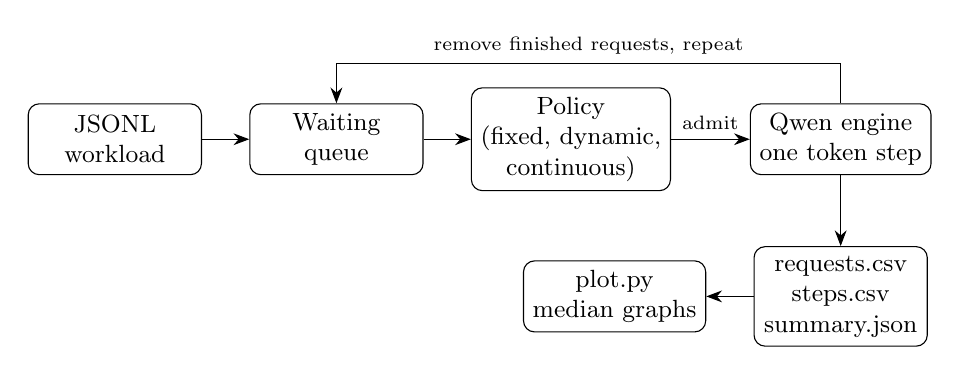
\begin{tikzpicture}[
    box/.style={draw, rounded corners, minimum height=0.9cm, minimum width=2.2cm, align=center, font=\small},
    arr/.style={-{Stealth[length=2mm]}}
]
\node[box] (wl) {JSONL\\workload};
\node[box, right=0.6cm of wl] (q) {Waiting\\queue};
\node[box, right=0.6cm of q] (pol) {Policy\\(fixed, dynamic,\\continuous)};
\node[box, right=1.0cm of pol] (eng) {Qwen engine\\one token step};
\node[box, below=0.9cm of eng] (out) {requests.csv\\steps.csv\\summary.json};
\node[box, left=0.6cm of out] (plot) {plot.py\\median graphs};
\draw[arr] (wl) -- (q);
\draw[arr] (q) -- (pol);
\draw[arr] (pol) -- node[above, font=\scriptsize]{admit} (eng);
\draw[arr] (eng) -- (out);
\draw[arr] (out) -- (plot);
\draw[arr] (eng.north) -- ++(0,0.5) -| node[above, pos=0.25, font=\scriptsize]{remove finished requests, repeat} (q.north);
\end{tikzpicture}
\caption{Benchmark data flow for one strategy run}
\label{fig:arch}
\end{figure}

\subsection{Batching strategies}
All three strategies use a maximum batch size of $B = 4$.

\begin{enumerate}
    \item \textbf{Fixed batching.} The policy waits until four requests are in the queue. Then it starts a closed batch and runs it until all four requests finish. The last batch can be smaller if the workload has no more requests.
    \item \textbf{Dynamic batching.} The policy starts a closed batch when four requests are in the queue or when the oldest waiting request has waited 50 ms. The batch then stays closed until all its requests finish.
    \item \textbf{Continuous batching.} After every token step, the policy fills each free slot from the waiting queue. It admits $\min(B - \text{active},\ \text{waiting})$ requests. It never waits on purpose.
\end{enumerate}

Each policy is a short Python class in \texttt{src/batch\_bench/schedulers.py}. The shared scheduler loop checks that no request is lost or counted twice after every admission and every step.

\subsection{Inference engine}
The engine in \texttt{src/batch\_bench/model.py} left-pads the active sequences to the same length, builds an attention mask and position IDs, and runs one forward pass. It takes the most probable next token for each sequence (greedy decoding). A request finishes when it reaches its \texttt{max\_new\_tokens} limit or produces an end-of-sequence token. Before the timed run starts, the engine does a warm-up pass and resets the CUDA peak-memory counter.

\subsection{Technology stack}
\begin{table}[H]
\centering
\caption{Software and model}
\begin{tabular}{ll}
\toprule
\textbf{Component} & \textbf{Version} \\
\midrule
Language & Python 3.11 \\
Deep learning library & PyTorch 2.8.0 with CUDA 12.8 \\
Model library & Hugging Face Transformers 4.46.3 \\
Model & \texttt{Qwen/Qwen2.5-0.5B-Instruct}, FP16 \\
Container & Docker 29.8.2 and Docker Compose, NVIDIA GPU runtime \\
Base image & \texttt{pytorch/pytorch:2.8.0-cuda12.8-cudnn9-runtime} \\
Graphs & Matplotlib 3.9.2 \\
\bottomrule
\end{tabular}
\end{table}

\section{Workflow}
One command runs the full experiment:
\begin{verbatim}
docker compose run --rm benchmark
\end{verbatim}

Docker Compose starts \texttt{python -m batch\_bench.experiment} inside the container. This script runs the dense workload first and the sparse workload second. For each workload, it calls \texttt{run.py} with three repetitions.

\texttt{run.py} starts a new child process for each strategy. The processes run one after the other, so two strategies never share the GPU. The strategy order rotates between repetitions (fixed, dynamic, continuous; then dynamic, continuous, fixed; and so on). This rotation reduces bias from GPU temperature or clock changes.

Each child process loads the model, does the warm-up pass, reads the workload, and runs the scheduler loop until all requests finish. It then writes three files:
\begin{itemize}
    \item \texttt{requests.csv}, one row per request with arrival, start, first-token, and finish times,
    \item \texttt{steps.csv}, one row per token step with the active batch size,
    \item \texttt{summary.json}, the percentiles, throughput, and peak CUDA memory for the run.
\end{itemize}

After each child exits, \texttt{run.py} checks that the result contains every request ID from the workload exactly once. When all runs finish, \texttt{plot.py} reads the three repetitions and draws the graphs.

\section{Experimental setup}

\subsection{Hardware}
\begin{itemize}
    \item \textbf{GPU:} NVIDIA GeForce RTX 5050 Laptop GPU, 8151 MiB, driver 592.82.
    \item \textbf{CPU:} 13th Gen Intel Core i7-13620H.
    \item \textbf{RAM:} 23.6 GiB.
    \item \textbf{Operating system:} Windows 11 Home, Docker Desktop with the NVIDIA runtime.
    \item \textbf{Power:} AC power, Windows ``High performance'' power plan.
\end{itemize}
The run happened on October 10, 2026. The model loaded from a local Hugging Face cache with \texttt{HF\_HUB\_OFFLINE=1}, so network speed did not affect the timings.

\subsection{Workloads}
Both workloads use the same 30 prompts and the same output limits. Only the gap between arrivals changes.

\begin{table}[H]
\centering
\caption{Workloads}
\begin{tabular}{lccc}
\toprule
\textbf{Workload} & \textbf{Requests} & \textbf{Arrival gap} & \textbf{Output limits (tokens)} \\
\midrule
Dense & 30 & 20 ms & 16, 32, 48 \\
Sparse & 30 & 400 ms & 16, 32, 48 \\
\bottomrule
\end{tabular}
\end{table}

In the dense workload, requests arrive faster than the GPU finishes them, so a queue builds up. In the sparse workload, requests arrive slowly. This shows the cost of waiting for a full batch.

\subsection{Metrics}
Let $a_i$ be the scheduled arrival time of request $i$, $f_i$ the time of its first output token, and $e_i$ the time of its last output token. Then:
\begin{align*}
\text{Latency}_i &= e_i - a_i \\
\text{TTFT}_i &= f_i - a_i \\
\text{Throughput} &= \frac{\sum_i \text{output tokens}_i}{\max_i e_i - \min_i a_i}
\end{align*}
Latency and TTFT start at the scheduled arrival, so both include time spent in the queue. The throughput denominator is the makespan of the whole run. In the sparse workload, it includes the planned gaps between arrivals.

Each strategy ran three times on each workload, which gives 18 runs. For every metric, we report the median of the three per-run values. Error bars on the graphs span the minimum and maximum run. Every run completed all 30 requests and produced exactly 960 output tokens, so all strategies did the same work.

\subsection{Choice of dynamic wait limit}
Before the main run, we did one run of each strategy at dynamic wait limits of 25, 50, 100, 200, and 400 ms. Table~\ref{tab:sweep} shows the dynamic results.

\begin{table}[H]
\centering
\caption{Dynamic batching wait-limit sweep (one run each)}
\label{tab:sweep}
\small
\begin{tabular}{lcccc}
\toprule
\textbf{Wait (ms)} & \textbf{Dense tok/s} & \textbf{Dense lat. p50} & \textbf{Sparse lat. p50} & \textbf{Sparse lat. p95} \\
\midrule
25 & 111.86 & 4483.39 & 1290.14 & 1890.20 \\
50 & 109.32 & 4085.01 & 1237.79 & 1561.65 \\
100 & 109.98 & 3947.56 & 1259.46 & 1722.86 \\
200 & 104.87 & 4141.50 & 1573.81 & 1656.57 \\
400 & 112.99 & 3909.86 & 1231.56 & 1904.19 \\
\bottomrule
\end{tabular}
\\[2pt]
{\small Latency in milliseconds.}
\end{table}

50 ms gave the lowest sparse p95 latency, so we used it for the main run. This sweep used the same workloads as the main run. It is tuning, not an independent test, and 50 ms may not be the best value for other workloads. An earlier full run at 25 ms is kept in \path{docs/results/windows-rtx-5050-2026-10-10/} for comparison.

\section{Results}
All numbers below are medians of three runs. Lower latency and TTFT are better. Higher throughput is better. The raw data for every run is in this repository folder:
\begin{center}
\path{docs/results/windows-rtx-5050-2026-10-10-wait50/}
\end{center}

\subsection{Dense workload}

\begin{table}[H]
\centering
\caption{Dense workload results}
\label{tab:dense}
\small
\setlength{\tabcolsep}{4pt}
\begin{tabular}{lcccccc}
\toprule
\textbf{Strategy} & \textbf{Tok/s} & \textbf{Lat. p50} & \textbf{Lat. p95} & \textbf{TTFT p50} & \textbf{TTFT p95} & \textbf{Avg. batch} \\
\midrule
Fixed & 111.89 & 3934.17 & 7387.23 & 3102.88 & 6557.84 & 2.50 \\
Dynamic & 113.84 & 4118.91 & 7310.49 & 3462.63 & 6759.23 & 2.50 \\
Continuous & \textbf{154.40} & \textbf{3082.77} & \textbf{5290.92} & \textbf{2150.59} & \textbf{4390.52} & \textbf{3.71} \\
\bottomrule
\end{tabular}
\\[2pt]
{\small Latency and TTFT in milliseconds.}
\end{table}

\begin{figure}[H]
    \centering
    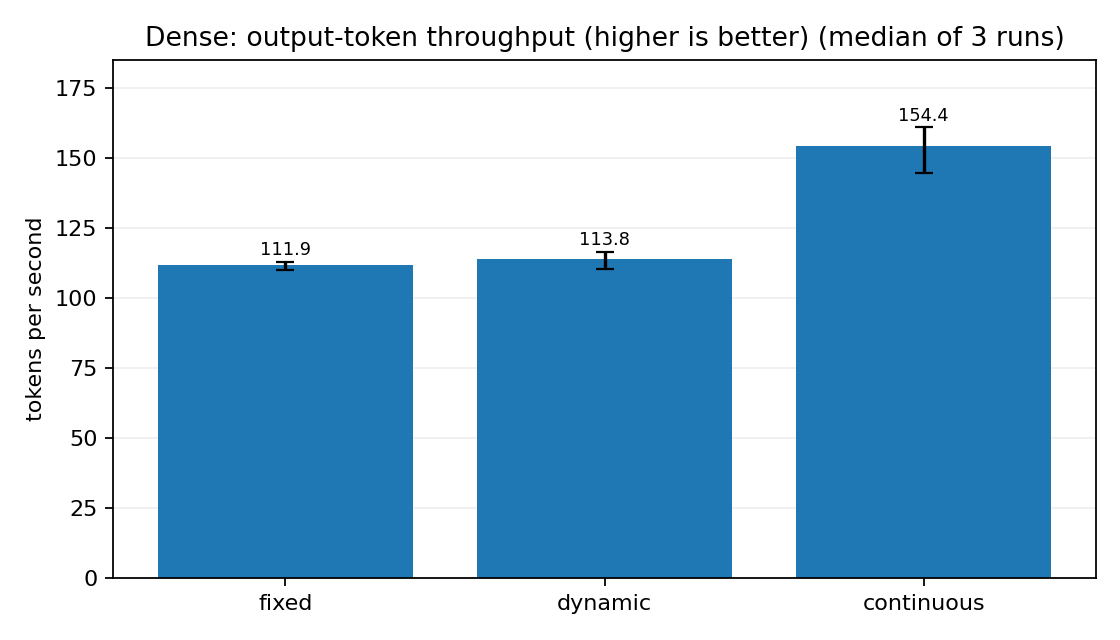
\includegraphics[width=0.8\textwidth]{figures/dense_throughput.png}
    \caption{Dense workload: output-token throughput}
    \label{fig:dense_tp}
\end{figure}

\begin{figure}[H]
    \centering
    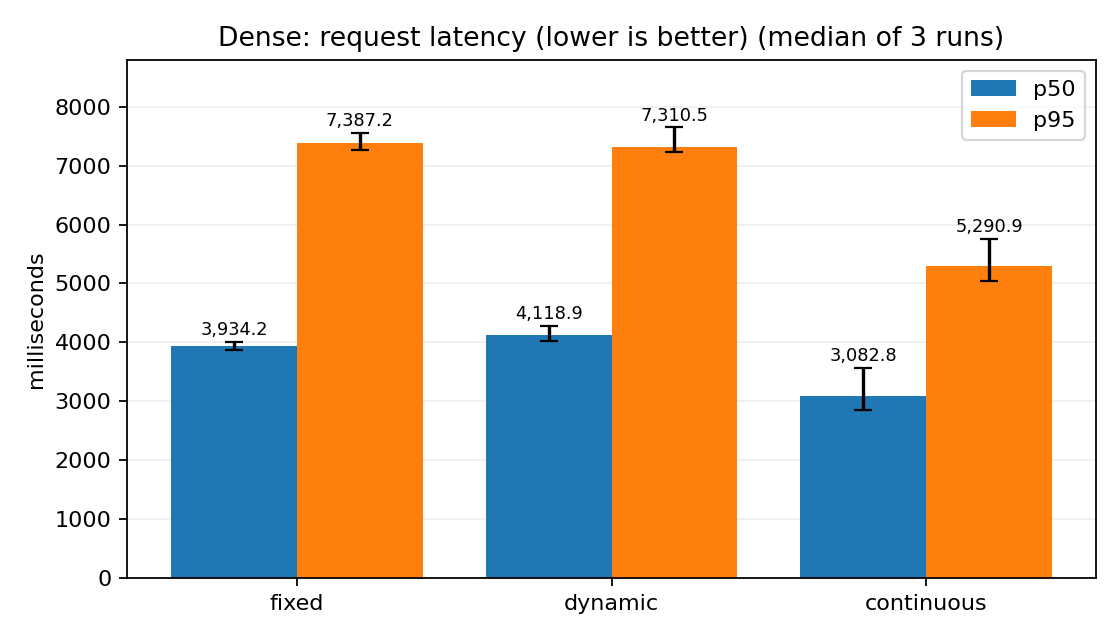
\includegraphics[width=0.8\textwidth]{figures/dense_latency.png}
    \caption{Dense workload: request latency}
    \label{fig:dense_lat}
\end{figure}

\begin{figure}[H]
    \centering
    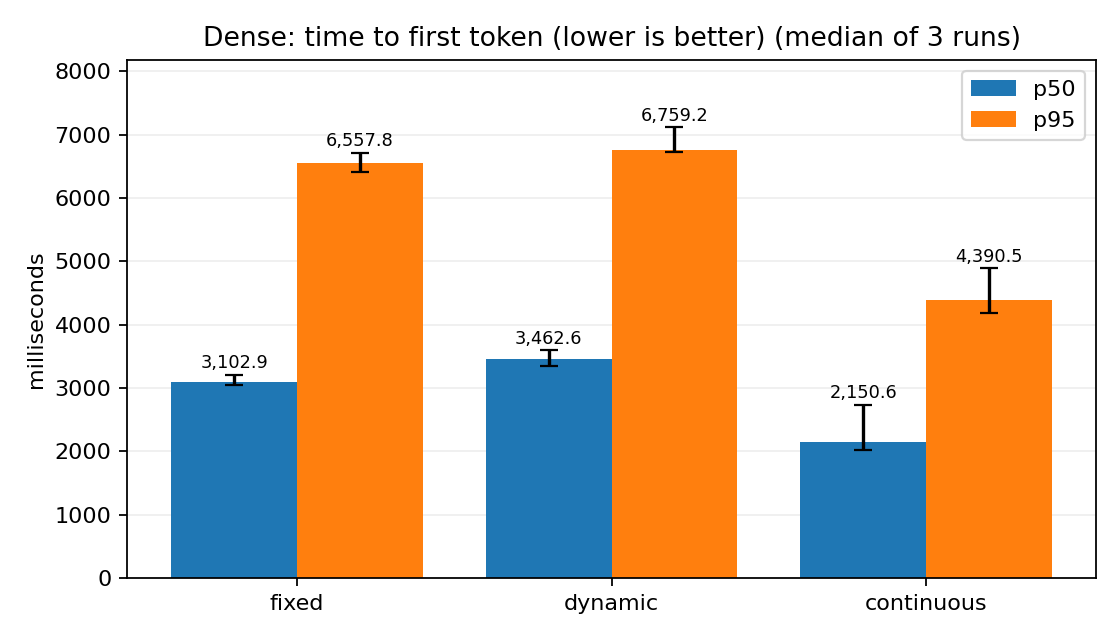
\includegraphics[width=0.8\textwidth]{figures/dense_ttft.png}
    \caption{Dense workload: time to first token}
    \label{fig:dense_ttft}
\end{figure}

\begin{figure}[H]
    \centering
    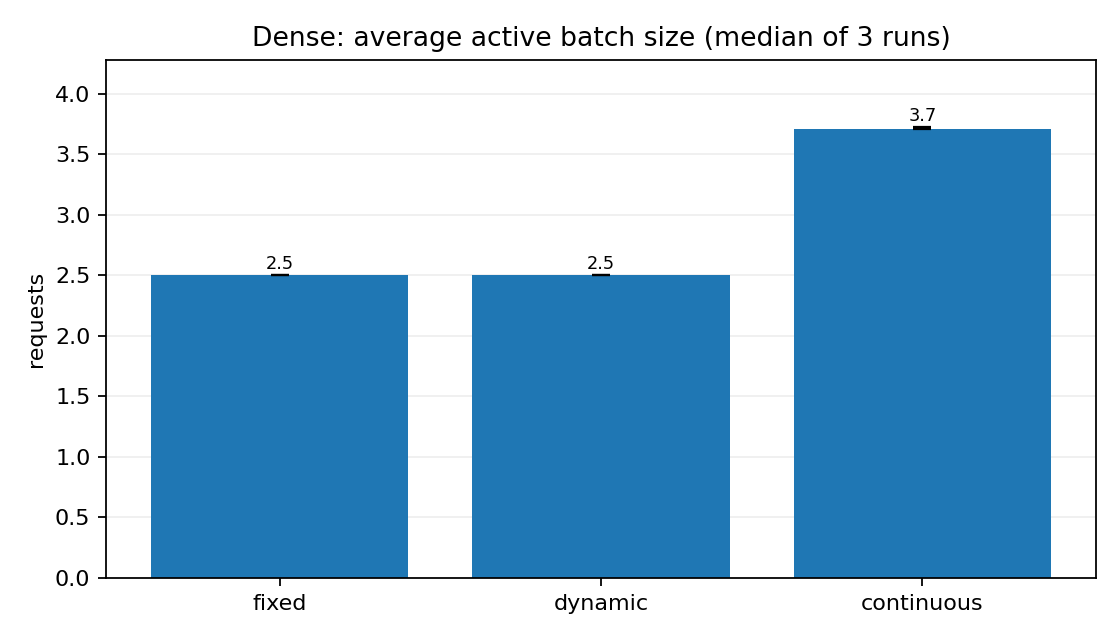
\includegraphics[width=0.8\textwidth]{figures/dense_batch_size.png}
    \caption{Dense workload: average active batch size}
    \label{fig:dense_bs}
\end{figure}

Continuous batching won every dense metric. Its throughput was 154.40 tokens/s against 111.89 for fixed, which is 38\% higher. Its p95 latency was 28\% lower and its p50 TTFT was 31\% lower.

The batch-size graph explains why. Fixed and dynamic batches start with four requests, but the requests have output limits of 16, 32, and 48 tokens. The short requests finish first and their slots stay empty until the longest one ends. The average active batch therefore drops to 2.50. Continuous batching refills a slot on the next step, so its average stayed at 3.71 out of 4. More active requests per step means more tokens for each forward pass.

Dynamic batching did not help under dense arrivals. While the GPU is busy, the queue grows, so four or more requests are usually waiting when a batch ends. The 50 ms deadline seldom fires and dynamic acts almost like fixed. Its median TTFT was 12\% worse than fixed. When the deadline does fire, dynamic starts a smaller closed batch, and the requests that arrive just after must wait for that whole batch to finish.

\subsection{Sparse workload}

\begin{table}[H]
\centering
\caption{Sparse workload results}
\label{tab:sparse}
\small
\setlength{\tabcolsep}{4pt}
\begin{tabular}{lcccccc}
\toprule
\textbf{Strategy} & \textbf{Tok/s} & \textbf{Lat. p50} & \textbf{Lat. p95} & \textbf{TTFT p50} & \textbf{TTFT p95} & \textbf{Avg. batch} \\
\midrule
Fixed & 73.91 & 1506.56 & 2184.72 & 586.26 & 1226.80 & 2.50 \\
Dynamic & 73.42 & 1256.70 & 1590.78 & 477.85 & 993.06 & 1.62 \\
Continuous & \textbf{75.94} & \textbf{736.47} & \textbf{1151.14} & \textbf{34.53} & \textbf{45.51} & 1.76 \\
\bottomrule
\end{tabular}
\\[2pt]
{\small Latency and TTFT in milliseconds.}
\end{table}

\begin{figure}[H]
    \centering
    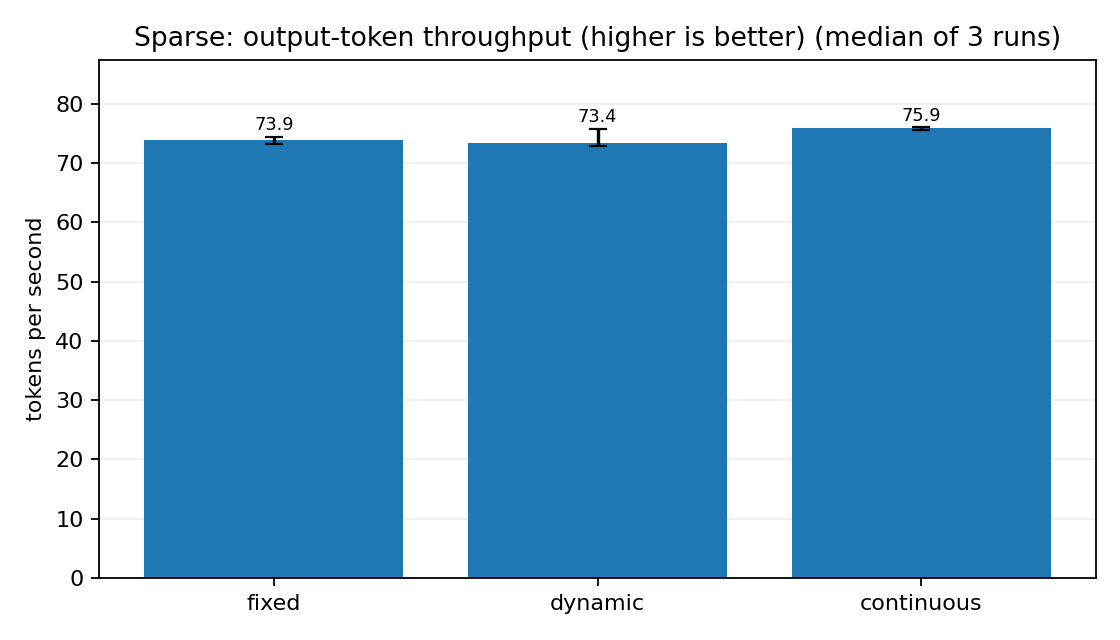
\includegraphics[width=0.8\textwidth]{figures/sparse_throughput.png}
    \caption{Sparse workload: output-token throughput}
    \label{fig:sparse_tp}
\end{figure}

\begin{figure}[H]
    \centering
    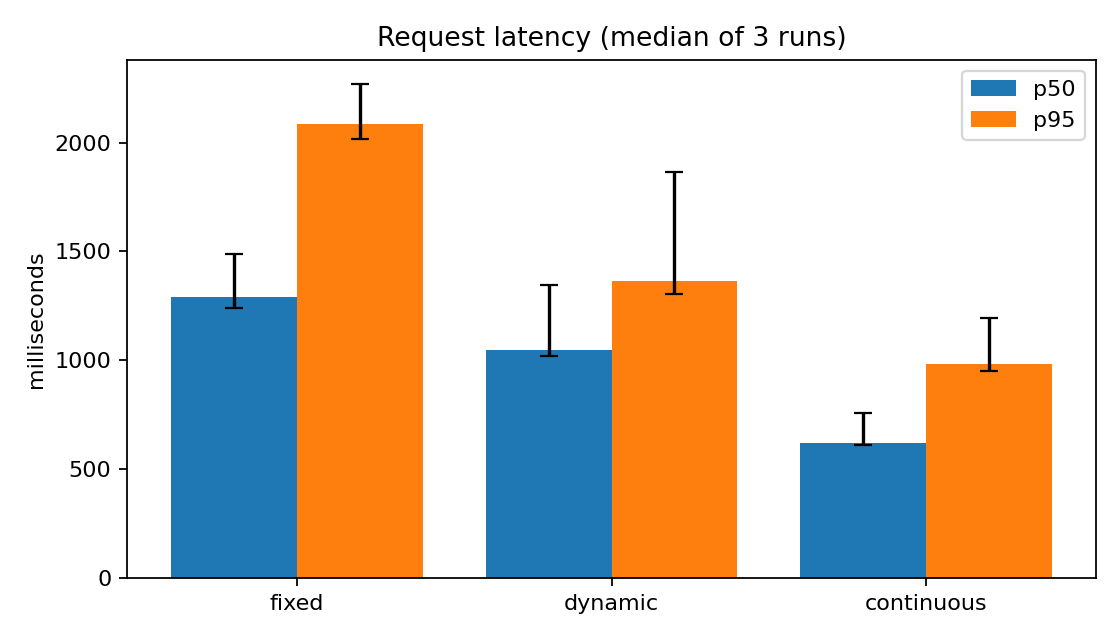
\includegraphics[width=0.8\textwidth]{figures/sparse_latency.png}
    \caption{Sparse workload: request latency}
    \label{fig:sparse_lat}
\end{figure}

\begin{figure}[H]
    \centering
    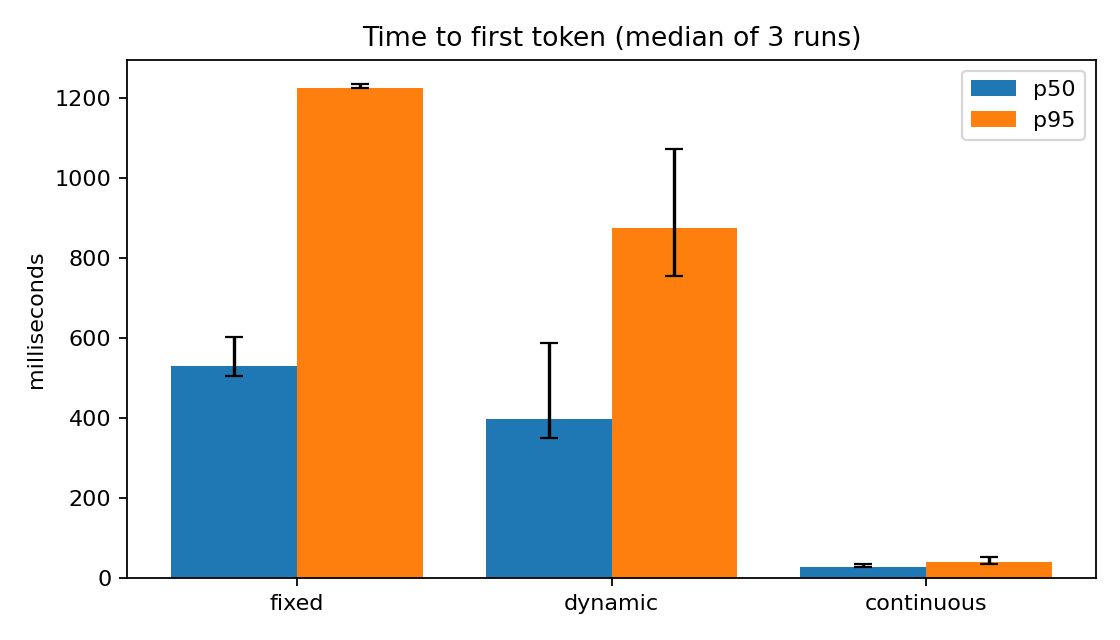
\includegraphics[width=0.8\textwidth]{figures/sparse_ttft.png}
    \caption{Sparse workload: time to first token}
    \label{fig:sparse_ttft}
\end{figure}

\begin{figure}[H]
    \centering
    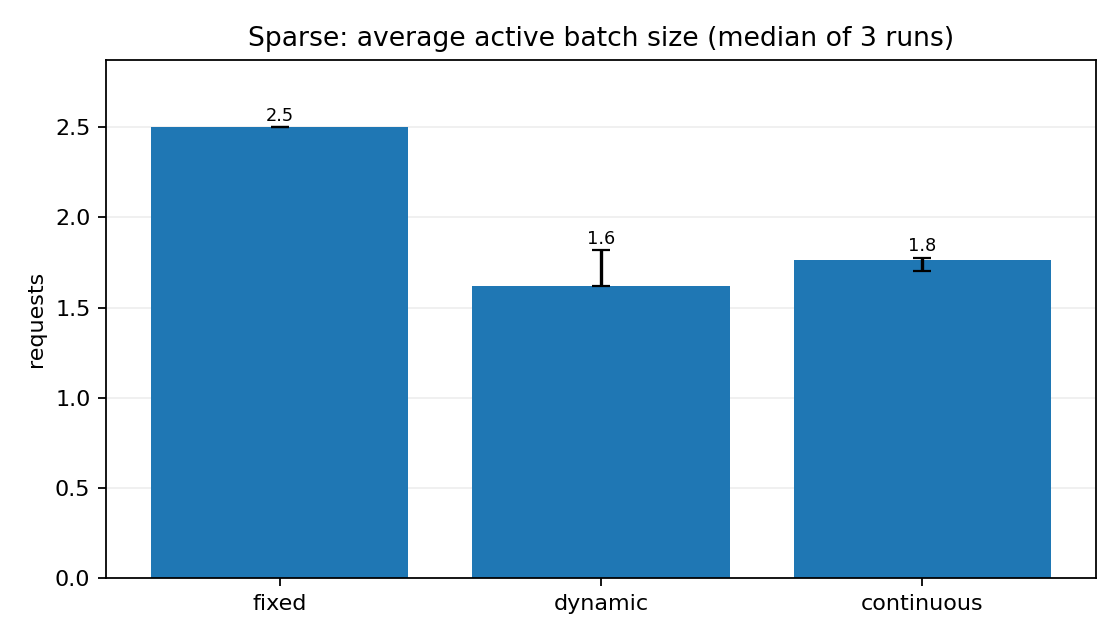
\includegraphics[width=0.8\textwidth]{figures/sparse_batch_size.png}
    \caption{Sparse workload: average active batch size}
    \label{fig:sparse_bs}
\end{figure}

Throughput was almost equal for all three strategies, between 73.42 and 75.94 tokens/s. The arrival schedule sets this number, not the scheduler. The last request arrives at 11.6 s, and the median makespan of each strategy was between 12.6 s and 13.1 s.

Latency is where the strategies differ. Fixed batching waits for four requests. At a 400 ms gap, that wait is up to 1.2 s, and the TTFT graph shows it. Dynamic batching cuts the wait at 50 ms. Compared with fixed, it lowered p50 latency by 17\%, p95 latency by 27\%, p50 TTFT by 18\%, and p95 TTFT by 19\%. Continuous batching admits each request on the next step after it arrives. Its p50 TTFT was 34.53 ms, which is 17 times lower than fixed. Its p50 latency was 736.47 ms, about half of the fixed value.

The continuous TTFT bars in Figure~\ref{fig:sparse_ttft} are small but not zero. They look flat because the same axis also shows fixed and dynamic values above 900 ms. The numbers on the bars give the exact values.

The average batch size of continuous (1.76) is smaller than fixed (2.50) in this workload. This is the expected trade. Fixed fills its batches by making requests wait. Continuous starts work at once with fewer requests on the GPU, and the arrival rate is too low to fill more slots.

\subsection{GPU memory}
Table~\ref{tab:mem} gives the median peak CUDA memory that PyTorch allocated after warm-up.

\begin{table}[H]
\centering
\caption{Peak allocated CUDA memory (MiB, median of three runs)}
\label{tab:mem}
\begin{tabular}{lccc}
\toprule
\textbf{Workload} & \textbf{Fixed} & \textbf{Dynamic} & \textbf{Continuous} \\
\midrule
Dense & 993.29 & 993.29 & 1023.61 \\
Sparse & 993.29 & 982.44 & 990.95 \\
\bottomrule
\end{tabular}
\end{table}

Every peak stayed near 1 GiB. Continuous batching used 30 MiB more under dense load because it kept more sequences active. This PyTorch counter does not include the CUDA context or driver memory. Even with those added, the benchmark fits the 3 to 4 GB VRAM target for this assignment.

\section{Limitations}
The engine runs real Qwen inference, but it calls the model with \texttt{use\_cache=False}. At each token step, it recomputes attention over the full prompt and all earlier output tokens. A production server keeps a KV cache and computes only the new token.

We chose this on purpose. All three strategies use the same inference path, so no strategy gets a faster model or a different memory policy. The difference in the results comes only from the admission rule. The cost is that each step does more work than necessary, so absolute latency and throughput are worse than a real server would give.

With a KV cache, every step would be faster, and all the absolute numbers would change. Cache memory would also grow with the number of active sequences, so memory would become part of the scheduling decision. We expect continuous batching to keep its lead, because the slot-refill effect does not depend on the step cost. The size of the gaps would change, though, and we did not measure it.

Other limits:
\begin{itemize}
    \item We tested one model, one GPU, one batch size ($B = 4$), and two arrival patterns.
    \item The 50 ms dynamic wait limit was tuned on the same workloads we report.
    \item Three repetitions show the spread between runs but are not enough for strong statistical tests.
    \item We did not implement PagedAttention, preemption, or multi-GPU execution.
\end{itemize}

\section{Conclusion}
Continuous batching gave the best result on both workloads in our setup. Under dense load, it raised throughput by 38\% because it kept 3.71 of 4 slots busy, against 2.50 for the closed-batch strategies. Under sparse load, it cut the median time to first token from 586 ms to 35 ms because no request waited for a batch to fill.

Dynamic batching is a partial fix. Its deadline helped under sparse arrivals, where it cut p95 latency by 27\% compared with fixed. Under dense arrivals, it behaved like fixed batching because it still keeps each batch closed until the longest request ends.

The main lesson for us is that the closed batch is the real problem, not the batch size. Fixed and dynamic batching differ only in when a batch starts. Both waste slots after short requests finish. ORCA's step-level admission removes that waste, and our measurements on a 0.5B model show the effect clearly even at batch size 4.

\begin{thebibliography}{9}
\bibitem{orca} G.-I. Yu, J. S. Jeong, G.-W. Kim, S. Kim, and B.-G. Chun. ORCA: A Distributed Serving System for Transformer-Based Generative Models. In \emph{16th USENIX Symposium on Operating Systems Design and Implementation (OSDI 22)}, 2022. \url{https://www.usenix.org/conference/osdi22/presentation/yu}
\bibitem{vllm} W. Kwon et al. Efficient Memory Management for Large Language Model Serving with PagedAttention. In \emph{SOSP 2023}. Source: \url{https://github.com/vllm-project/vllm}
\bibitem{qwen} Qwen Team. Qwen2.5-0.5B-Instruct model card. \url{https://huggingface.co/Qwen/Qwen2.5-0.5B-Instruct}
\bibitem{hf} Hugging Face. Transformers documentation. \url{https://huggingface.co/docs/transformers}
\bibitem{torch} PyTorch documentation. \url{https://pytorch.org/docs/stable/}
\bibitem{docker} Docker documentation. \url{https://docs.docker.com/}
\end{thebibliography}

\end{document}
